\documentclass[../../main.tex]{subfiles}

\begin{document}

\chapter{Árvore rubro-negra} \label{cap:rubronegra}

Iremos implementar uma árvore rubro-negra utilizando a técnica de Node copying, discutida na Seção~\ref{sec:nodecopying}. Uma árvore rubro-negra é uma árvore de busca binária balanceada, na qual cada nó é vermelho ou preto, e as cores são usadas para auxiliar no rebalanceamento.

Com uma implementação baseada na de Cormen et. al~\cite{CormenRedBlack}, a cada inserção ou remoção em uma árvore de~$n$ nós, são necessárias apenas~$\Oh(1)$ rotações para rebalancear a árvore, e~$\Oh(\lg n)$ mudanças de cores. Como as cores servem apenas para auxiliar no rebalanceamento, não é necessário que estes dados persistam, ou seja, só precisamos saber a cor dos nós ativos, logo apenas~$\Oh(1)$ passos de modificação~(considerando apenas os ponteiros de filho esquerdo e direito de um nó) por inserção, logo esta implementação parcialmente persistente consome tempo~$\Oh((m + a) \lg(m))$ e espaço~$\Oh(m)$, onde~$m$ é o número de operações de modificação~(inserções e remoções), e~$a$ é o número de operações de acesso~(acessar um elemento, seu teto ou chão, mínimo, etc.).

A implementação de Sedgewick e Wayne~\cite{SedgewickRedBlack}, apesar de ser considerada mais simples, não serve para os nossos propósitos, pois, ao considerar apenas árvores rubro-negras esquerdistas, os algoritmos de inserção e remoção podem realizar~$\Theta(\lg n)$ rotações, logo não é possível manter o consumo de espaço~$\Oh(m)$.

Se~$\Oh(m \lg m)$ de espaço é aceitável, uma implementação funcional garante esse espaço, e é totalmente persistente. Esse método é discutido na Seção~\ref{sec:implfuncional}, e também usado nos capítulos~\ref{cap:pilha},~\ref{cap:deque1},~\ref{cap:deque2} e~\ref{cap:deque3}.

\section{Definições}

Uma árvore de busca binária é uma árvore em que cada nó possui um valor, e tem no máximo dois filhos (esquerdo e direito). Para todo nó, o valor de todos os nós em sua subárvore esquerda é menor ou igual ao seu valor, e o valor de todos os nós em sua subárvore direita é maior ou igual ao seu valor.

Um nó que não tem algum filho armazena~\keyword{null} no campo correspondente a esse filho. Uma folha é um nó que não tem filhos, e um link nulo é um campo de filho de algum nó que tem valor~\keyword{null}, na Figura~\ref{fig:arv_bin_ex} são as arestas tracejadas.

\begin{figure}
\centering
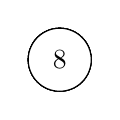
\begin{tikzpicture}[
nodes = {draw, circle, minimum size = 8mm},
edge from parent path = {(\tikzparentnode) -- (\tikzchildnode)},
sibling distance=20pt,
ed/.style = {densely dashed, shorten >= 5pt},
n/.style = {draw=none},
r/.style = {fill=white},
b/.style = {fill=gray},
edge from parent/.append style={-, shorten >= 0, shorten <= 0}]
\Tree [.\node[b]{7}; [.\node[b]{5}; [.\node[r]{1}; \edge[ed];\node[n]{}; \edge[ed];\node[n]{}; ] \edge[ed];[.\node[n]{}; ] ] [.\node[b]{10}; [.\node[r]{8}; \edge[ed];\node[n]{}; \edge[ed];\node[n]{}; ] \edge[ed];[.\node[n]{}; ] ] ]
\end{tikzpicture}
\caption{Exemplo de árvore rubro-negra. Como no resto das figuras do capítulo, os nós negros tem fundo cinza e os nós vermelhos tem fundo branco. Nas próximas figuras, o valor de cada nó não é especificado.} \label{fig:arv_bin_ex}
\end{figure}

Uma árvore rubro-negra segue as seguintes propriedades:
\begin{enumerate}
\item A raiz é preta.
\item Se um nó é vermelho, este não tem filhos vermelhos.
\item Para todo nó, todos os caminhos até links nulos de sua subárvore têm o mesmo número de nós pretos.
\end{enumerate}

Considerando apenas os nós pretos, a árvore é totalmente balanceada (propriedade 3). Como um nó vermelho não tem filhos vermelhos (propriedade 2), é possível ``juntar'' os nós vermelhos aos seus pais pretos (a raiz não é vermelha pela propriedade 1), e assim cada nó preto fica associado até~3 valores. Logo, um simples limitante superior para a altura de uma árvore rubro-negra de~$n$ nós é~$3\floor{\lg(n)}$. Se mantivermos essas propriedades a cada inserção ou remoção, e o consumo de tempo destas for proporcional à altura da árvore, então o consumo de tempo será~$\Oh(\lg n)$ para todas as operações.

\section{Implementação da persistência}

\newcommand{\ts}{\mathcal{T}}
\renewcommand{\copy}{\V{copy}}
\newcommand{\child}{\V{child}}
\newcommand{\parent}{\V{parent}}
\newcommand{\red}{\V{red}}
\newcommand{\extra}{\V{extra}}
\newcommand{\eSide}{\V{extraSide}}
\newcommand{\eTs}{\V{extra\mathcal{T}}}
\newcommand{\version}{\V{version}}
\newcommand{\side}{\V{side}}
\newcommand{\roots}{\V{roots}}
\newcommand{\val}{\V{value}}


Em uma árvore rubro-negra efêmera, todo nó precisa de dois campos para seus filhos, e um valor booleano que indica se o nó é vermelho. Como já discutido, o campo booleano não precisa ser guardado de forma persistente. Como cada nó tem grau de entrada no máximo~1, no nó persistente é necessário armazenar apenas um ponteiro de volta e um ponteiro extra. O ponteiro de volta é armazenado no campo~$\parent$, e é exatamente o ponteiro que aponta para o pai de um nó, o que será conveniente durante a implementação das operações. Note que, de acordo com a implementação da Seção~\ref{sec:nodecopying}, o campo~$\parent$ é nulo para nós que não são ativos, logo não pode ser utilizado para realizar as operações de acesso.

Para evitar a necessidade de replicar código muito parecido, vamos armazenar os filhos como um vetor~$\child$ de~2 posições,~$u.\child[0]$ é o filho esquerdo de~$u$, e~$u.\child[1]$ é seu filho direito. Os campos de um nó serão:
\begin{itemize}
\item $\ts$ --- Tempo de criação do nó.
\item $\copy$ --- Próximo nó persistente (se este não é ativo).
\item $\child$ --- Vetor de filhos.
\item $\parent$ --- Ponteiro de volta.
\item $\red$ --- Booleano que indica se o nó é vermelho.
\item $\extra, \eSide, \eTs$ --- Ponteiro extra, seu lado e tempo de modificação.
\item $\val$ --- O valor armazenado pelo nó
\end{itemize}

Note que é necessário armazenar~$\eSide$, o lado do ponteiro extra, pois ele pode ser tanto um filho esquerdo quanto direito do nó, e se~$\extra$ for nulo, não há como saber qual filho este é comparando seu valor com o do nó. Para indicar se o ponteiro extra foi utilizado, usaremos que~$\ts = -1$ quando não existe tal ponteiro.

\section{Operações de acesso}

Para acessar o campo de um nó na versão~$\version$, usamos uma versão modificada da função~\textsc{Access}.


\begin{algorithm}
\begin{algorithmic}[1]

\Require $u$ deve ser um nó persistente associado à versão~$\version$.
\Function{ChildAt}{$u, \side, \version$}
	\If{$u.\eTs \neq -1 \And u.\eSide = \side \And \version \geq u.\eTs$}
		\State \Return $u.\extra$
	\EndIf
	\State \Return $u.\child[\side]$
\EndFunction

\end{algorithmic}
\end{algorithm}

Vamos apresentar a operação de~\textsc{Find}, que retorna o valor buscado, ou~\keyword{null} se ele não foi encontrado. Assumimos que é guardado um vetor~$\roots$, com o nó de entrada (a raiz) para cada versão.

\begin{algorithm}
\begin{algorithmic}[1]

\Function{Find}{$x, \version$}
	\State $u = \roots[\version]$
	\While{$u \neq \Null \And x \neq u.\val$}
	\State $u = \Call{ChildAt}{u, [x > u.\val], \version}$ \label{line:findrb:iver}
	\EndWhile
	\If{$u = \Null$}
		\State \Return \Null
	\Else
		\State \Return $x.\val$
	\EndIf
\EndFunction

\end{algorithmic}
\end{algorithm}

O algoritmo funciona como em uma árvore efêmera, mas usando a função~\textsc{ChildAt} para acessar o filho direito ou esquerdo, em vez de utilizar o campo~$\child$, que pode não ter a versão desejada do ponteiro. Note que, na linha~\nref{line:findrb:iver}, já utilizamos a notação de~Iverson para diminuir o código. Outras operações de acesso (chão e teto, por exemplo) podem ser implementadas da mesma forma.

\section{Modificação de um campo}

Vamos apresentar as funções~\textsc{Modify} e~\textsc{Copy}, adaptadas da Seção~\ref{sec:nodecopying}, para utilizar durante as operações de modificação. Usamos que apenas ponteiros são modificados em uma árvore rubro-negra.

\begin{algorithm}
\begin{algorithmic}[1]

\Function{Modify}{$u, \side, v, \version$}
	\If{$u.\copy \neq \Null$}
		\State $u = u.\copy$
	\EndIf
	\If{$u.\version < \version$}
		\State $u.\copy = \Call{Copy}{u, \version}$
		\State $u = u.\copy$
	\EndIf
	\If{$u.\child[\side] \neq \Null$}
		\State $u.\child[\side].\parent = \Null$
	\EndIf
	\State $u.\child[\side] = v$
	\If{$v \neq \Null$}
		\State $v.\parent = u$
	\EndIf
\EndFunction

\Function{Copy}{$u, \version$}
	\State $u' = \Call{RawCopy}{u}$
	\If{$u.\eTs \neq -1$}
		\State $u'.\child[u.\eSide] = u.\extra$
		\State $u'.\eTs = -1$ \Comment{Limpando o campo extra}
	\EndIf
	\State $u'.\ts = \version$
	\State $u.\parent = \Null$
	\If{$\roots[\version] = u$}
		\State $\roots[\version] = u'$
	\EndIf
	\For{$\side \in \{0, 1\}$}
		\If{$u'.\child[\side] \neq \Null$}
			\State $u'.\child[\side].\parent = u'$
		\EndIf
	\EndFor
	\If{$u'.\parent \neq \Null$}
		\State $v = u'.\parent$
		\State $\side = [u'.\val > v.\val]$
		\If{$v.\ts = \version$}
			\State $v.\child[\side] = u'$
		\ElsIf{$v.\eTs = -1$}
			\State $v.\eTs = \version$
			\State $v.\extra = u'$
			\State $v.\eSide = \side$
		\Else
			\State $v.\copy = \Call{Copy}{v, \version}$
			\State $v.\child[\side] = u'$
		\EndIf
	\EndIf
	\State \Return $u'$
\EndFunction

\end{algorithmic}
\end{algorithm}

Utilizamos que cada nó tem apenas um campo extra e ponteiro de volta para diminuir o código, e o vetor de filhos para evitar duplicação de código. Com estas funções prontas, é possível manter a persistência da estrutura, e nas próximas seções vamos discutir como implementar as operações de inserir e remover um valor de uma árvore rubro-negra.

\section{Inserção}

TODO



\end{document}
